\section{Experimental Results} \label{sec:results}

We evaluate the effectiveness of DeepTune for two distinct OpenCL optimization
tasks: predicting the optimal device to use to run a given OpenCL program, and
predicting thread coarsening factors.

We first compare DeepTune against two expert-tuned predictive models, showing
that DeepTune outperforms the state-of-the-art in both cases. We then show that
by leveraging knowledge learned from training DeepTune for one heuristic, we can
boost training for the other heuristic, further improving performance. Finally,
we analyze the working mechanism of DeepTune.


\subsection{Case Study A: OpenCL Heterogeneous Mapping}

Selecting the optimal execution device for OpenCL kernels is essential for
maximizing performance. For a CPU/GPU heterogeneous system, this presents a
binary choice. In this experiment, we compare our approach against a static
single-device approach and the Grewe \emph{et al.\ }predictive model. The
\emph{static mapping} selects the device which gave the best average case
performance over all the programs. On the AMD platform, the best-performing
device is the CPU; on the NVIDIA platform, it is the GPU.

Figure~\ref{fig:cgo-accuracy} shows the accuracy of both predictive models and
the static mapping approach for each of the benchmark suites. The static
approach is accurate for only 58.8\% of cases on AMD and 56.9\% on NVIDIA. This
suggests the need for choosing the execution device on a per program basis. The
Grewe \emph{et al.\ }model achieves an average accuracy of 73\%, a significant
improvement over the static mapping approach. By automatically extracting useful
feature representations from the source code, DeepTune gives an average accuracy
of 82\%, an improvement over the other two schemes.

Using the static mapping as a baseline, we compute the relative performance of
each program using the device selected by the Grewe \emph{et al.\ }and DeepTune
models. Figure~\ref{fig:cgo-speedup} shows these speedups. Both predictive
models significantly outperform the static mapping; the Grewe \emph{et al.\
}model achieves an average speedup of $2.91\times$ on AMD and $1.26\times$ on
NVIDIA (geomean $1.18\times$). In 90\% of cases, DeepTune matches or outperforms
the predictions of the Grewe \emph{et al.\ }model, achieving an average speedup
of $3.34\times$ on AMD and $1.41\times$ on NVIDIA (geomean $1.31\times$). This
14\% improvement in performance comes at a greatly reduced cost, requiring no
intervention by humans.

\begin{figure}
  \centering %
  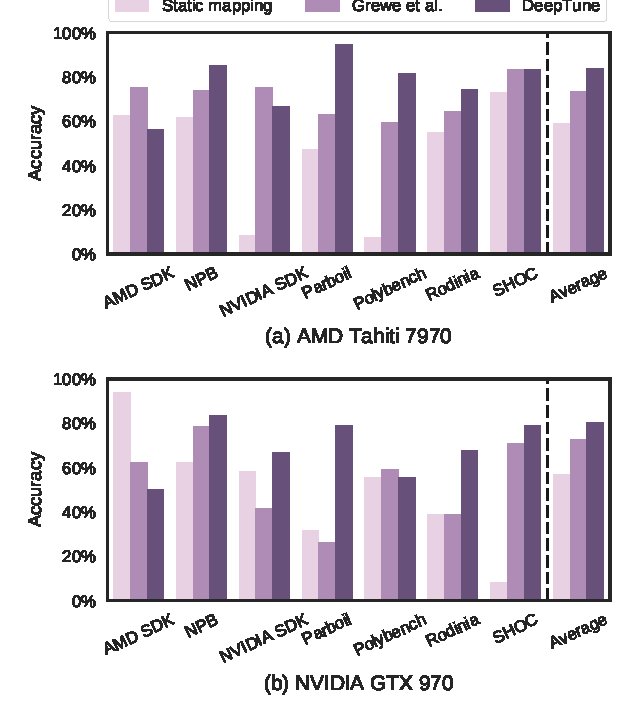
\includegraphics[width=\columnwidth]{img/cgo-acc}%
  \caption{%
    Accuracy of optimization heuristics for heterogeneous device mapping,
    aggregated by benchmark suite. The optimal static mapping achieves 58\%
    accuracy. The Grewe \emph{et al.\ }and DeepTune predictive models achieve
    accuracies of 73\% and 84\%, respectively.%
  }
  \label{fig:cgo-accuracy}
\end{figure}

\begin{figure*}
  \centering %
  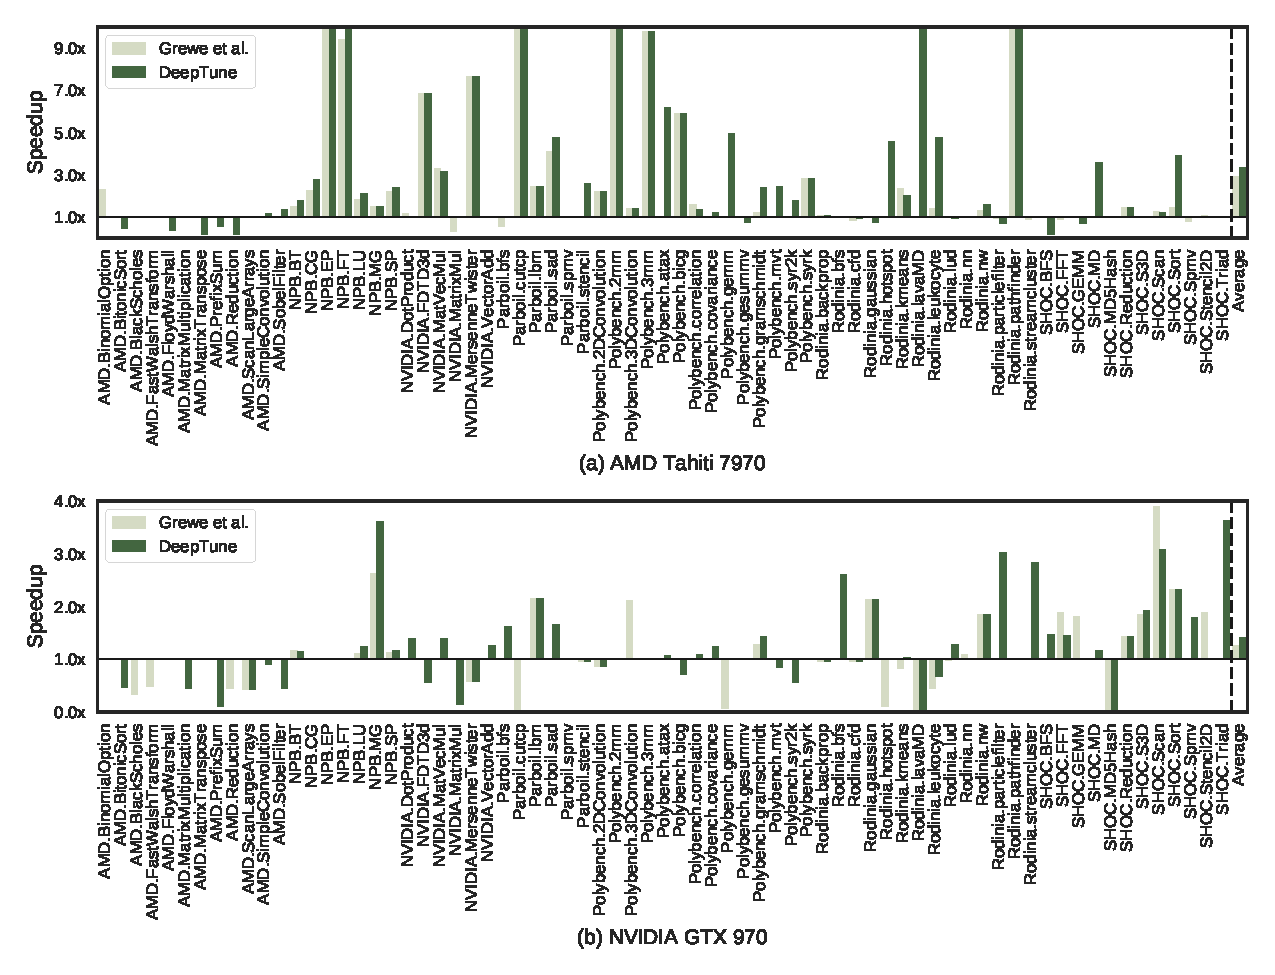
\includegraphics[width=\textwidth]{img/cgo-speedup}%
  \vspace{-1em}
  \caption{%
    Speedup of predicted heterogeneous mappings over the best static mapping for
    both platforms. In (a) DeepTune achieves an average speedup of 3.43x over
    static mapping and 18\% over Grewe \emph{et al}. In (b) the speedup is 1.42x
    and 13\% respectively.%
  }
  \label{fig:cgo-speedup} %
\end{figure*}



\subsection{Case Study B: OpenCL Thread Coarsening Factor}

\begin{figure*}
  \centering %
  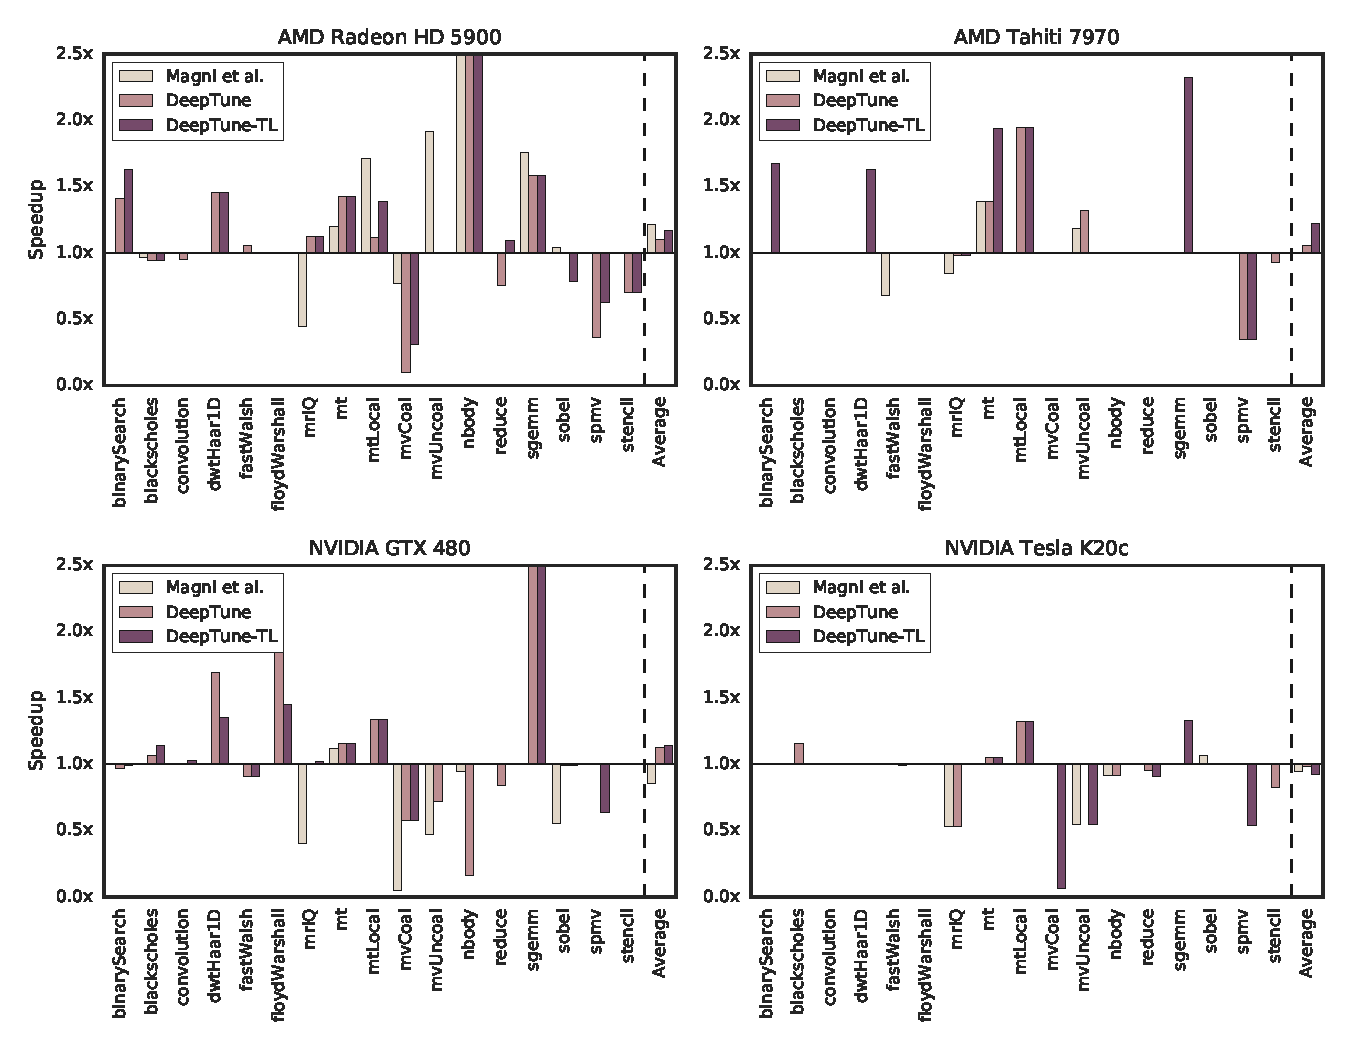
\includegraphics[width=\textwidth]{img/pact-speedup}%
  \vspace{-1em}
  \caption{%
    Speedups of predicted coarsening factors for each platform. DeepTune
    outperforms Magni \emph{et al} on three of the four platforms. Transfer
    learning improves DeepTune speedups further, by 16\% on average.%
  }%
  \label{fig:pact-speedup} %
\end{figure*}


Exploiting thread coarsening for OpenCL kernels is a difficult task. On average,
coarsening slows programs down. The maximum speedup attainable by a perfect
heuristic is $1.36\times$.

Figure~\ref{fig:pact-speedup} shows speedups achieved by the Magni \emph{et al.\
}and DeepTune models for all programs and platforms. We use as baseline the
performance of programs without coarsening.  On the four experimental platforms
(AMD HD 5900, Tahiti 7970, NVIDIA GTX 480, and Tesla K20c), the Magni \emph{et
al.\ }model achieves average speedups of $1.21\times$, $1.01\times$,
$0.86\times$, and $0.94\times$, respectively. DeepTune outperforms this,
achieving speedups of $1.10\times$, $1.05\times$, $1.10\times$, and
$0.99\times$.

Some programs --- especially those with large divergent regions or indirect
memory accesses --- respond very poorly to coarsening. No performance
improvement is possible on the \texttt{mvCoal} and \texttt{spmv} programs. Both
models fail to achieve positive average speedups on the NVIDIA Tesla K20c,
because thread coarsening does not give performance gains for the majority of
the programs on this platform.

The disappointing results for both predictive models can be attributed to the
small training program set used by Magni \emph{et al.\ }(only 17 programs in
total). As a result, the models suffer from sparse training data. Prior research
has shown that data sparsity can be overcome using additional programs; in the
following subsection we describe and test a novel strategy for training
optimization heuristics on a small number of programs by exploiting knowledge
learned from other optimization domains.


\subsection{Transfer Learning Across Problem Domains}\label{subsec:tl}

There are inherent differences between the tasks of building heuristics for
heterogeneous mapping and thread coarsening, evidenced by the contrasting
choices of features and models in Grewe \emph{et al.\ }and Magni \emph{et al.\ }
However, in both cases, the first role of DeepTune is to extract meaningful
abstractions and representations of OpenCL code. Prior research in deep learning
has shown that models trained on similar inputs for different tasks often share
useful commonalities. The idea is that in neural network classification,
information learned at the early layers of neural networks (i.e. closer to the
input layer) will be useful for multiple tasks. The later the network layers are
(i.e. closer to the output layer), the more specialized the layers
become~\cite{Zeiler2014}.

We hypothesized that this would be the case for DeepTune, enabling the novel
transfer of information between models \emph{across different optimization
domains}. To test this, we extracted the language model --- the
\texttt{Embedding}, \texttt{LSTM\_1}, and \texttt{LSTM\_2} layers --- trained
for the heterogeneous mapping task and \emph{transferred} it over to the new
task of thread coarsening. Since DeepTune keeps the same design for both
optimization problems, this is as simple as copying the learned weights of the
three layers. Then we trained the model as normal.

As shown in Figure~\ref{fig:pact-speedup}, our newly trained model, DeepTune-TL
has improved performance for 3 of the 4 platforms: $1.17\times$, $1.23\times$,
$1.14\times$, $0.93\times$, providing an average 12\% performance improvement
over Magni \emph{et al.}  In 81\% of cases, the use of transfer learning matched
or improved the optimization decisions of DeepTune, providing up to a 16\%
improvement in per platform performance.

On the NVIDIA Tesla K20c, the platform for which no predictive model achieves
positive average speedups, we match or improve performance in the majority of
cases, but over-coarsening on three of the programs causes a modest reduction in
average performance. We suspect that for this platform, further performance
results are necessary due to its unusual optimization profile.


\subsection{DeepTune Internal Activation States}

\begin{figure*}
  \centering %
  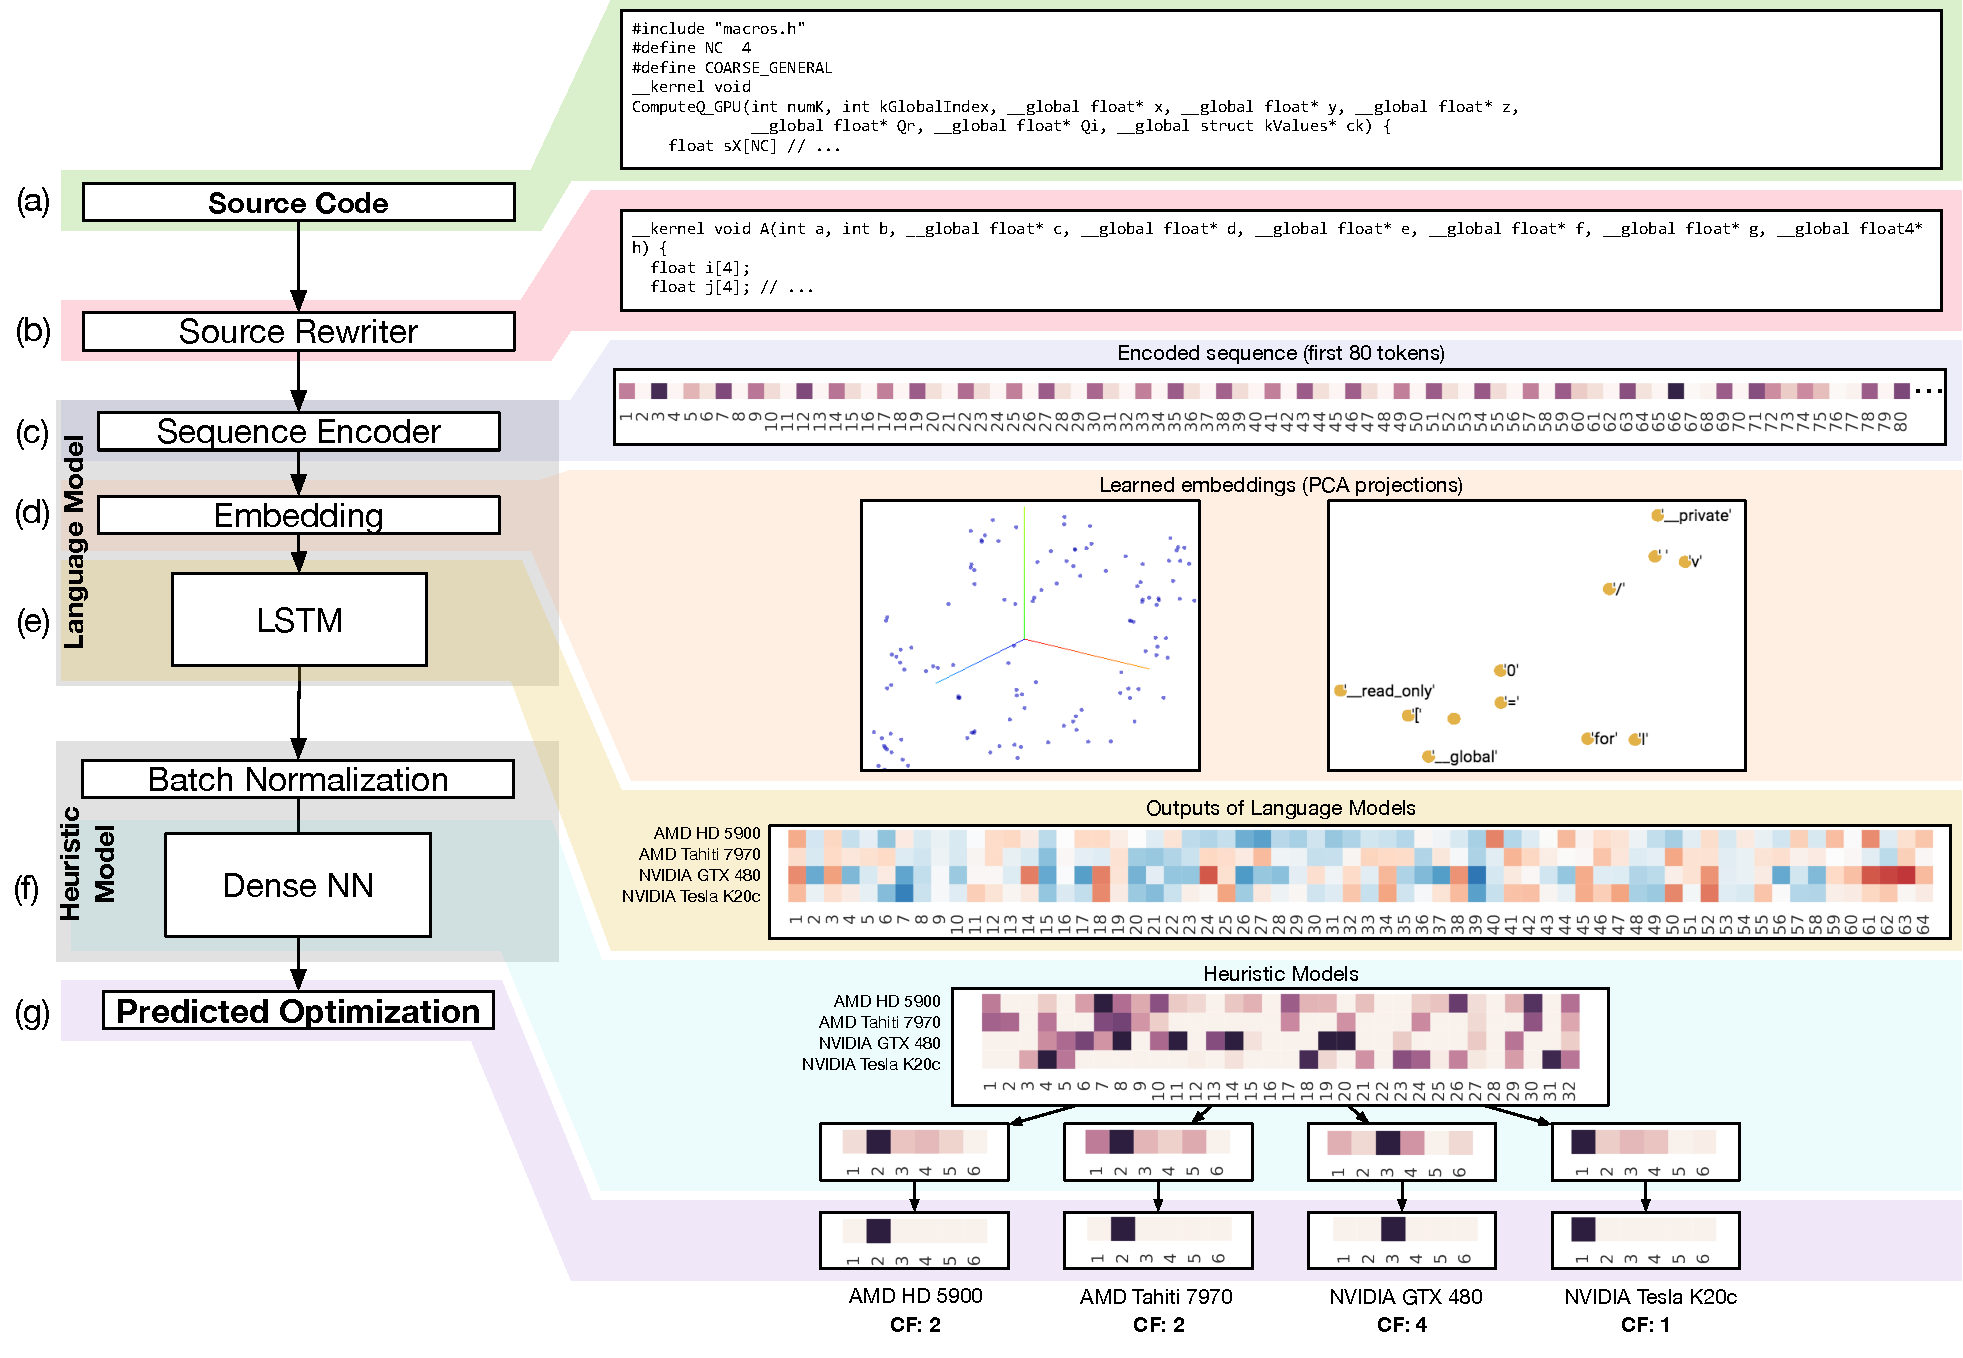
\includegraphics[width=\textwidth]{img/viz}%
    \vspace{-1em}
  \caption{%
    Visualizing the internal state of DeepTune when predicting coarsening factor
    for Parboil's \texttt{mriQ} benchmark on four different architectures. The
    activations in each layer of the four models increasingly diverge the lower
    down the network.%
  }
  \label{fig:viz} %
\end{figure*}


We have shown that DeepTune automatically outperforms state-of-the-art
predictive models for which experts have invested a great amount of time in
engineering features. In this subsection we attempt to illuminate the inner
workings, using a single example from Case Study B: predicting the thread
coarsening factor for Parboil's \texttt{mriQ} benchmark on four different
platforms.

Figure~\ref{fig:viz} shows the DeepTune configuration, with visual overlays
showing the internal state. From top to bottom, we begin first with the input,
which is the 267 lines of OpenCL code for the \texttt{mriQ} kernel. This source
code is preprocessed, formatted, and rewritten using variable and function
renaming, shown in Figure~\ref{fig:viz}b. The rewritten source code is tokenized
and encoded in a $1$-of-$k$ vocabulary. Figure~\ref{fig:viz}c shows the first 80
elements of this encoded sequence as a heatmap in which each cell's color
reflects its encoded value. The input, rewriting, and encoding is the same for
each of the four platforms.

The encoded sequences are then passed into the Embedding layer. This maps each
token of the vocabulary to a point in a 64 dimension vector space. Embeddings
are learned during training so as to cluster semantically related tokens
together. As such, they may differ between the four platforms.
Figure~\ref{fig:viz}d shows a PCA projection of the embedding space for one of
the platforms, showing multiple clusters of tokens. By honing in on one of the
clusters and annotating each point with its corresponding token, we see that the
cluster contains the semantically related OpenCL address space modifiers
\texttt{\_\_private}, \texttt{\_\_global}, and \texttt{\_\_read\_only}.

Two layers of 64 LSTM neurons model the sequence of embeddings, with the neuron
activations of the second layer being used to characterize the entire sequence.
Figure~\ref{fig:viz}e shows the neurons in this layer for each of the four
platforms, using a red-blue heatmap to visualize the intensity of each
activation. Comparing the activations between the four platforms, we note a
number of neurons in the layer with different responses across platforms. This
indicates that the language model is partly specialized to the target platform.

As information flows through the network, the layers become progressively more
specialized to the specific platform. We see this in Figure~\ref{fig:viz}f,
which shows the two layers of the heuristic model. The activations within these
increasingly diverge. The mean variance of activations across platforms
increases threefold compared to the language model, from 0.039 to 0.107. Even
the activations of the AMD HD 5900 and AMD Tahiti 7970 platforms are dissimilar,
despite the final predicted coarsening factor for both platforms being the same.
In Figure~\ref{fig:viz}g we take the largest activation of the output layer as
the final predicted coarsening factor. For this particular program, a state-of-
the-art model achieves 54\% of the maximum performance. DeepTune achieves 99\%.
